\providedisablepart{showscreenshot}
\begin{frame}[fragile]
    \frametitle{Example: Translation}
    \begin{itemize}
        \item Two German words for \str{cousin}, depending on the gender
        \item Two entries in abstract syntax: \verb|cousin_female| and \verb|cousin_male|
        \item Use inference to discard ASTs
    \end{itemize}
    
    \vspace{2em}
    \small
    \begin{minipage}[t][5cm]{\textwidth}
        \begin{tikzpicture}
            \node(eng) at (-4,1) {\parbox{4.2cm}{\str{Kim is Ahmed's cousin and the father of Grace}}};
                \node(ger1) at (-4,-0.5) {\parbox{4.2cm}{\str{Kim ist Ahmeds {\upshape\bf Cousine} und Graces Vater}}};
                \node(ger2) at (-4,-2.0) {\parbox{4.2cm}{\str{Kim ist Ahmeds {\upshape\bf Cousin} und Graces Vater}}};
            \node(ast1) at (0,1) {AST$_1$};
            \node(ast2) at (0,-1) {AST$_2$};
            \only<2->{
                \node(log1) at (3,1) {\color{logicfont} \parbox{2.2cm}{$female(kim) \wedge$ $male(kim)$}};
                \node(log2) at (3,-1) {\color{logicfont} \parbox{2.2cm}{$male(kim) \wedge$ $male(kim)$}};
            }
            \draw[->,thick] (eng) -- (ast1);
            \draw[->,thick] (eng) -- (ast2);
                \draw[->,thick] (ast1) -- (ger1);
                \draw[->,thick] (ast2) -- (ger2);
            \only<2->{
                \draw[->,thick] (ast1) -- (log1);
                \draw[->,thick] (ast2) -- (log2);
            }
            \only<3>{
                \draw[ultra thick,red] (2,1.5) -- (4,0.5);
                \draw[ultra thick,red] (2,0.5) -- (4,1.5);
                
                \draw[ultra thick,red] (-0.5,1.5) -- (0.5,0.5);
                \draw[ultra thick,red] (-0.5,0.5) -- (0.5,1.5);

                \draw[ultra thick,red] (-6,0.0) -- (-2,-1.0);
                \draw[ultra thick,red] (-6,-1.0) -- (-2,0.0);
            }
        \end{tikzpicture}
    \end{minipage}
    \ifpart{showscreenshot}{\only<4>{
        \begin{tikzpicture}[overlay,remember picture]
            \fill[gray!80,opacity=0.8] (current page.north west) rectangle (current page.south east);
            \node at (current page.center) { 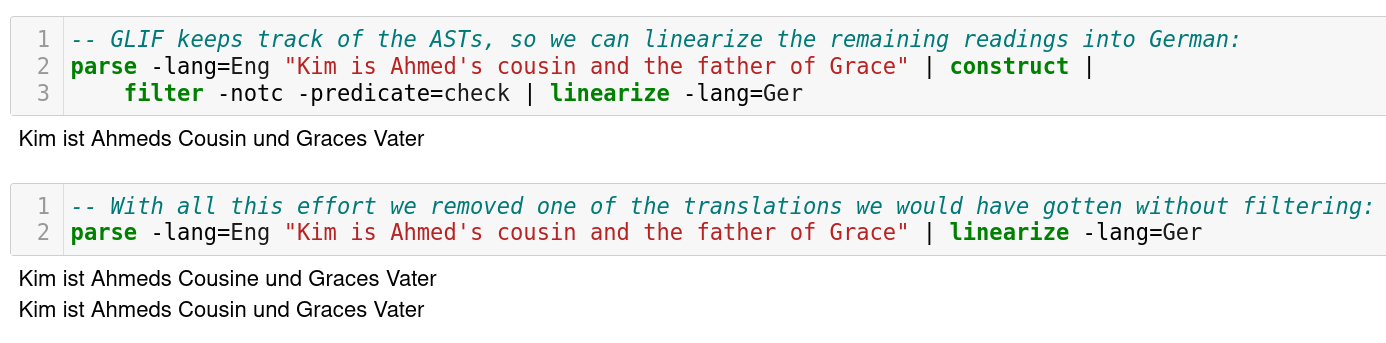
\includegraphics[width=\textwidth]{img/screenshot-glif-5.png} };
        \end{tikzpicture}
    }}{}
\end{frame}
